\section{Lensing noise bias}

We now consider weak gravitational lensing of the 21--cm signal by the large scale structure, as a source of noise in searches for magnetic fields using the method proposed in this work. We first compute the transverse shear power spectrum and then evaluate the noise bias it produces for the magnetic--field estimator. We demonstrate that this bias is very small, even for arrays with futuristic collecting areas of one hundred square kilometers.

To follow standard lensing notation, we no longer label cartesian coordinate axes with $x$, $y$, and $z$, but rather with numbers, using the convention where directions $1$ and $2$ lie in the plane of the sky, while $3$ lies along the line of sight. Specifically, we use angular coordinates $(\theta_1, \theta_2)$ to denote direction in the sky ${\bf{\widehat n}}$, and $\theta_3$ to denote a comoving interval $r_z/\chi(z)$ along the line of sight, located at redshift $z$, and corresponding to $\Delta z$ interval. As before, we denote variables in Fourier space with tilde. We use $\vec{\ell}\equiv(\ell_1,\ell_2)$ for a conjugate variable of ${\bf{\widehat n}}$. 
 
We start by generalizing the formalism for two--dimensional weak lensing \cite{Weinberg201387} to the three--dimensional case.
In the presence of lensing, a source coordinate $\theta_i^S$, where $i\in\{1,2,3\}$, maps onto the observed coordinate $\theta_i$ as follows 
\beq
\theta_k^S=\theta_k+\frac{\partial\psi}{\partial\theta_k},\ k=1,2,\ \ \ \theta_3^S=\theta_3,
\label{eq:lensingmapping}
\eeq
where $\psi$ is the lensing potential. The full Jacobian of this coordinate transformation is
\beq
\bga
\mathcal{J}_{ij}\equiv\frac{\partial\theta_i^S}{\partial\theta_j}=\left(\begin{array}{ccc}
1+\psi_{,11} & \psi_{,12} & \psi_{,13}\\
\psi_{,21} & 1+\psi_{,22} & \psi_{,23}\\
0&0&1
\end{array}\right) \\
= \left(\begin{array}{ccc}
1+\kappa+\gamma_{11} & \gamma_{12} & \gamma_{13}\\
\gamma_{12} & 1+\kappa-\gamma_{11} & \gamma_{23}\\
0&0&1
\end{array}\right),
\ega
\label{eq:lensingtsf}
\eeq
where $i,j\in\{1,2,3\}$, and the commas stand for partial derivatives with respect to the corresponding coordinates, as usual. In the above Equation, $\kappa$ and $\gamma$ components represent the magnification and shear, respectively. Fourier transform of the lensing potential is
\begin{equation}
\widetilde{\psi}(\vec{\ell},z)\equiv\int\psi({\bf\widehat{n}},z)e^{-i\vec{\ell}\cdot{\bf{\widehat n}}}\ d\theta_1 d\theta_2,
\label{eq:potentialFourier}
\end{equation}
where the relation between $\psi({\bf\widehat{n}},z)$ and the Newtonian potential $\Phi$ in a flat universe reads
\begin{equation}
\psi({\bf{\widehat n}},z)=
-2\int_0^{\chi(z)}d\chi_1\left[\frac{1}{\chi_1}-\frac{1}{\chi}\right]\Phi({\bf{\widehat n}},\chi_1).
\label{eq:lensingpotential}
\end{equation}
Combining Eqs.~(\ref{eq:potentialFourier}) and (\ref{eq:lensingpotential}), we get 
\begin{equation}
\frac{\partial\widetilde{\psi}(\vec{\ell},z)}{\partial\theta_3}=-\frac{2}{\chi(z)}\int_0^{\chi(z)} d\chi_1\widetilde{\Phi}(\vec{\ell},\chi_1).
\label{eq:dpsi_dtheta3}
\end{equation}
From Eqs.~(\ref{eq:dpsi_dtheta3}) and (\ref{eq:lensingtsf}), it follows 
\beq
\bga
\langle\widetilde{\gamma}_{13}^*(\vec{\ell},z)\widetilde{\gamma}_{13}(\vec{\ell}',z')\rangle=\left\langle \ell_1\ell_1'\frac{\widetilde{\psi}^*(\vec{\ell},z)}{\partial\theta_3}\frac{\widetilde{\psi}(\vec{\ell}',z')}{\partial\theta_3}\right\rangle\\
=\frac{4\ell_1\ell_1'}{\chi(z)\chi(z')}\int_0^{\chi(z)}d\chi_1\int_0^{\chi(z')}d\chi_1'\langle\widetilde{\Phi}^*(\vec{\ell},\chi_1)\widetilde{\Phi}(\vec{\ell}',\chi_1')\rangle.
\ega
\eeq

We now define the three--dimensional Fourier transform $\widetilde{\widetilde\Phi}$ of the Newtonian potential,
\beq
\widetilde{\Phi}(\vec{\ell},\chi)\equiv\int\widetilde{\widetilde{\Phi}}(\vec{\ell},\ell_3)e^{i\ell_3\chi}\frac{d\ell_3}{2\pi}.
\eeq
Using this definition, we get
\beq
\bga
\langle\widetilde{\Phi}^*(\vec{\ell},\chi)\widetilde{\Phi}(\vec{\ell}',\chi')\rangle=\int\int\frac{d\ell_3}{2\pi}\frac{d\ell_3'}{2\pi}\langle\widetilde{\widetilde{\Phi}}^*(\vec{\ell},\ell_3)\widetilde{\widetilde{\Phi}}(\vec{\ell}',\ell_3')\rangle\\
\times e^{i(\ell_3'\chi'-\ell_3\chi)}. 
\ega
\label{eq:doubletilde}
\eeq
Assuming different modes are uncorrelated, we arrive at
\beq
\bga
\langle\widetilde{\widetilde{\Phi}}^*(\vec{\ell},\ell_3)\widetilde{\widetilde{\Phi}}(\vec{\ell}',\ell_3')\rangle\\
=(2\pi)^3\delta(\ell_3-\ell_3')\delta^2(\vec{\ell}-\vec{\ell}')P_{\Phi}(\sqrt{\ell_3^2+\ell^2}),
\ega
\label{eq:expectation_tildetildephi}
\eeq
where
\beq
\bga
P_{\Phi}(\ell)=\frac{P_{\Phi}(k=\ell/\chi(z))}{\chi(z)^2}\\
=\left[\frac{3}{2}\Omega_mH_0^2(1+z)\right]^2\frac{P_{\delta}(k,z)}{k^4\chi(z)^2}.
\ega
\eeq
Substituting Eq.~(\ref{eq:expectation_tildetildephi}) into (\ref{eq:doubletilde}) and applying Limber approximation $\ell_3\ll\ell$, we obtain
\beq
\bga
\langle\widetilde{\Phi}^*(\vec{\ell},\chi)\widetilde{\Phi}(\vec{\ell}',\chi')\rangle\\
=(2\pi)^2\delta(\vec{\ell}-\vec{\ell}')P_{\Phi}(\ell)\delta(\chi'-\chi).
\ega
\eeq
Thus, for $z\leq z'$,
\beq
\bga
\langle\widetilde{\gamma}_{13}^*(\vec{\ell},z)\widetilde{\gamma}_{13}(\vec{\ell}',z')\rangle\\
=\frac{4}{\chi(z)\chi(z')}\ell_1\ell_1'(2\pi)^2\delta^2(\vec{\ell}-\vec{\ell}')\int_0^{\chi(z)}d\chi_1P_{\Phi}(\ell).
\ega
\label{eq:exp_gamma13}
\eeq

We are interested in calculating the power spectrum $P_{13}(\vec{\ell},z,z')$ of $\gamma_{13}$ components, defined as
\beq
\bga
\langle\widetilde{\gamma}_{13}^*(\vec{\ell},z)\widetilde{\gamma}_{13}(\vec{\ell}',z')\rangle\\
\equiv(2\pi)^2P_{13}(\vec{\ell},z,z')\delta(\vec{\ell}-\vec{\ell}').
\ega
\eeq
From Eq.~(\ref{eq:exp_gamma13}), we can express
\beq
P_{13}(\vec{\ell},z,z')=\frac{4\ell_1^2}{\chi(z)\chi(z')}\int_0^{\chi(z)}d\chi_1P_{\Phi}(\ell).
\eeq
A similar result holds for the power spectrum $P_{23}$ of $\gamma_{23}$ component. The transverse power spectrum $P_t$ reads
\beq
\bga
P_t(\ell,z,z')\equiv P_{13}+P_{23}\\
=\frac{4\ell^2}{\chi(z)\chi(z')}\int_0^{\chi(z)}d\chi_1P_{\Phi}(\ell).
\ega
\eeq
If $z=z'$, the above expression simplifies to
\beq
P_t(\ell,z)=\frac{4\ell^2}{\chi(z)^2}\int_0^{\chi(z)}d\chi_1P_{\Phi}(\ell).
\label{eq:Pt}
\eeq

Now that we have computed the transverse power spectrum, we move on to evaluating the contamination it produces for the measurement of the magnetic field. Denoting a vector transpose with ``T'', let us set ${\bf{\widehat k}}=(\sin\theta\cos\phi,\sin\theta\sin\phi,\cos\theta)^{\rm T}$, and consider the line of sight along the direction 3, ${\bf{\widehat n}}=(0,0,1)^{\rm T}$, in the three--dimensional Cartesian reference frame where $x$, $y$, and $z$ axes correspond to 1, 2, and 3, respectively; $\theta$ is the angle between the direction 3 and ${\bf{\widehat k}}$. Lensing distorts ${\vec{k}}$ into
\beq
{\vec{k}}'=[\mathcal{J}^{-1}]^{\rm T}\cdot{\vec{k}}=\left(1-\frac{2\kappa}{3}\right){\vec{k}}+{\bm{\sigma}}\cdot{\vec{k}}+{\bf{\Omega}}\times{\vec{k}},
\label{eq:distorted_kn}
\eeq
where $\mathcal{J}$ is given by Eq.~(\ref{eq:lensingtsf}) and
\beq
\bga
\bm{\sigma}\equiv\left(\begin{array}{ccc}
-\kappa/3-\gamma_{11} & -\gamma_{12} & -\gamma_{13}/2 \\
-\gamma_{12} & -\kappa/3+\gamma_{11} & -\gamma_{23}/2 \\
-\gamma_{23}/2 & -\gamma_{23}/2 & 2\kappa/3
\end{array}\right),\\
\bm{\Omega}\equiv(-\gamma_{23}/2,\gamma_{13}/2,0)^{\rm T},
\ega
\eeq
where $\bm{\sigma}$ is a tensor quantity. The first term in Eq.~(\ref{eq:distorted_kn}) only changes the magnitude of ${\vec{k}}$, the third term only changes its direction, and the second term contributes to both changes. To leading order, the fractional magnitude change is
$(k'-k)/k=-2\kappa/3+\widehat{\bf{k}}\cdot\bm{\sigma}\cdot\widehat{\bf{k}}$.
We now define
\beq
C\equiv 26.4\ {\rm mK}\ \left(1-\frac{T_\gamma}{T_{\rm s}}\right)x_{\rm 1s}\left(\frac{1+z}{10}\right)^{1/2},
\eeq
and use Eqs.~(\ref{eq:distorted_kn}) and (\ref{eq:tbsoln}) to arrive at the expression for the brightness--temperature fluctuation in the presence of lensing (keeping only the leading--order terms and assuming no magnetic fields),
\beq
\bga
{T}_{\rm (lens)}(\widehat{\bf{n}},\vec{k})=\frac{1}{\det(\mathcal{J})} T\left(\widehat{\bf{n}},{\vec{k}}'\right)  \\
=T\left(\widehat{\bf{n}},{\vec{k}}\right)(1-2\kappa) +C\left\lbrace {\delta}({\vec{k}})2(\widehat{\bf{k}}\cdot\widehat{{\bf{n}}})\left[\widehat{{\bf{n}}}\cdot\bm{\sigma}\cdot\widehat{{\bf{k}}}\right.\right. \\
\left.\left.-(\widehat{\bf{k}}\cdot\widehat{{\bf{n}}})(\widehat{\bf{k}}\cdot\bm{\sigma}\cdot\widehat{{\bf{k}}})+(\bm{\Omega}\times\widehat{{\bf{k}}})\cdot\widehat{{\bf{n}}}\right]\right.\\
\left.+\left(-\frac{2\kappa}{3}{\vec{k}}+\bm{\sigma}\cdot{\vec{k}}
+\bm{\Omega}\times{\vec{k}}\right)\cdot\bm{\nabla}_{\vec{k}}{\delta}({\vec{k}})\left[1+(\widehat{\bf{k}}\cdot\widehat{{\bf{n}}})^2\right]\right\rbrace,
\ega
\eeq
where $\det(\mathcal{J})$ corresponds to the determinant of $\mathcal{J}$. The lensed signal power spectrum is then given by
\beq
\bga
P_{\rm (lens)}^S({\vec{k}})=C^2 P_{\delta}(k)\left(1+(\widehat{\bf{k}}\cdot\widehat{{\bf{n}}})^2\right) \\
\times\left\lbrace \left(1+(\widehat{\bf{k}}\cdot\widehat{{\bf{n}}})^2\right) \left[1-2\kappa\left(1+\frac{1}{3}\frac{\partial\ln P_\delta(k)}{\partial\ln k}\right)\right.\right.\\
\left.
+\frac{\partial\ln P_\delta(k)}{\partial\ln k}(\widehat{\bf{k}}\cdot\bm{\sigma}\cdot\widehat{{\bf{k}}})\right]
+4(\widehat{\bf{k}}\cdot\widehat{{\bf{n}}})\\
\left.\times\left(\left[\widehat{\bf{n}}-
(\widehat{\bf{k}}\cdot\widehat{{\bf{n}}})
\widehat{\bf{k}}\right]\cdot\bm{\sigma}\cdot\widehat{\bf{k}}
+(\bm{\Omega}\times\widehat{\bf{k}})\cdot\widehat{\bf{n}}\right)\right\rbrace,
\label{eq:Tb_power}
\ega
\eeq
where we use $\partial\ln P_\delta(k)/\partial\ln k\sim -2.15$ (the slope of the density--fluctuation power spectrum, evaluated at redshift and $k$ values that contribute most to the SNR for magnetic--field measurement). On the other hand, from Eq.~(\ref{eq:tbsoln}), a magnetic field contributes to the signal as
\beq
\bga
P_B^S({\vec{k}})=C^2 P_{\delta}(k)\left(1+(\widehat{\bf{k}}\cdot\widehat{{\bf{n}}})^2\right) \times\\
\left\lbrace \left(1+(\widehat{\bf{k}}\cdot\widehat{{\bf{n}}})^2\right) + 1.353\times 10^{16}\left(\frac{1+z}{10}\right)^{-1/2}\right. \\
\left.\times \frac{T_{\gamma}}{T_{\rm s}}\frac{x_{\rm 1s}}{(1+x_{\alpha,(2)}+x_{c,(2)})^2}\left[{\vec{B}}\cdot(\widehat{\bf{k}}\times\widehat{{\bf{n}}})\right](\widehat{\bf{k}}\cdot\widehat{{\bf{n}}})\right\rbrace,
\label{eq:Tbmag_power}
\ega
\eeq
where ${\vec{B}}$ is given in units of Gauss (physical, rather than comoving). Let us now consider a magnetic field in the $(1,2)$ plane, such that ${\vec{B}}=(B_x,B_y,0)$; the results will be valid for any field orientation. If we explicitly expand both Eq.~(\ref{eq:Tb_power}) and Eq.~(\ref{eq:Tbmag_power}) in terms of spherical harmonics, and consider only $Y_{2\pm 1}$ terms (which dominate the terms that are asymmetric around the line--of--sight direction; contribution from the higher--order harmonics is subdominant), we can match the coefficient of Eq.~(\ref{eq:Tb_power}) that corresponds to the multiplier to the magnetic--field strength of Eq.~(\ref{eq:Tbmag_power}). With this procedure, we arrive at the expression for the comoving value of the lensing--induced spurious magnetic field given by 
\beq
\bga
{\vec{B}}_{\rm (lens)}=1.577\times 10^{-18}{\left[\rm Gauss\right]}\ \times \frac{1}{x_{\rm 1s}}\left(\frac{T_s}{T_{\gamma}}\right)\left(\frac{1+z}{10}\right)^{-3/2}\\
\times(1+x_{\alpha,(2)}+x_{c,(2)})^2\left(1+\frac{11}{16}\frac{\partial\ln P_\delta(k)}{\partial\ln k}\right)\\
\times(-\gamma_{23},\gamma_{13},0)^{\rm T}
\equiv\alpha(-\gamma_{23},\gamma_{13},0)^{\rm T},
\label{eq:alpha_def}
\ega
\eeq
in units of comoving Gauss. The lensing noise bias for magnetic--field reconstruction reads
\beq
P_{(\text{lens})}^{\rm noise}(\ell)=P_{(\text{lens})}^{\rm noise, B_x}+P_{(\text{lens})}^{\rm noise, B_y}=\alpha^2 P_t(\ell),
\eeq
where $\alpha$ is given by Eq.~(\ref{eq:alpha_def}) and $P_t(\ell)$ is given by Eq.~(\ref{eq:Pt}). Finally, the root--mean--square of the contamination is given by
\beq
\Delta_{(\text{lens})}(\ell)=\sqrt{\frac{\ell(\ell+1)}{2\pi}P_{(\text{lens})}^{\rm noise}(\ell)}.
\label{eq:delta_lens}
\eeq

A survey of size 1 sr, considered in this work, corresponds to $\ell\sim 6$, which relates to the lensing--potential fluctuations on comoving scale $\ell/D(z)\sim 5\times 10^{-4}{\rm Mpc}^{-1}$ at $z\sim 20$. We evaluate the contamination of Eq.~(\ref{eq:delta_lens}) at this multipole, which has a dominant contribution to the noise bias.\footnote{Note that the derivations shown in this Appendix hold only if the scale of matter fluctuations that contribute most to the lensing contamination are much larger than than those that contribute the most SNR for magnetic--field measurements, which is indeed the case here.}, and show the results in Fig.~\ref{fig:lensing_B}. Comparing this to Fig.~\ref{fig:Bsat}, we see that the contamination due to lensing shear remains below the projected sensitivities even for the case of futuristic array sizes. It may further be possible to distinguish lensing contribution from that of a magnetic field using difference in shapes of the inferred signal power spectra, but such detailed considerations are beyond the scope of this work.
\begin{figure}[h]
\centering
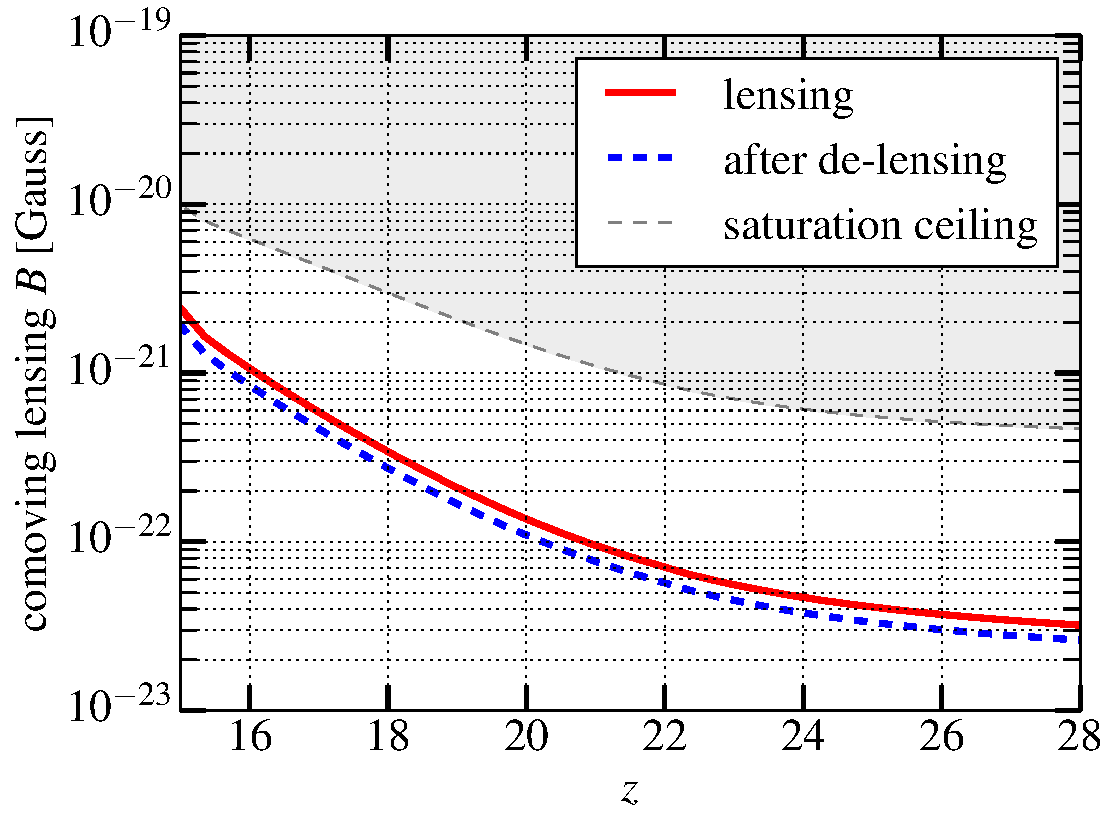
\includegraphics[scale=0.4]{delensingB.pdf}
\caption{The lensing--shear noise bias for the measurement of the magnetic field is shown before (solid red line) and after the de--lensing procedure is applied (dashed blue line). The saturation ceiling is denoted by the shaded region above the thin dashed line. Comparison with Fig.~\ref{fig:Bsat} reveals that lensing noise is below the projected sensitivity even for futuristic array sizes.}
\label{fig:lensing_B}
\end{figure}
